%%%%%%%%%%%%%%%%%%%%%%%%%%%%%%%%%%%%%%%%%%%%%%%%%%%%%%%%%%%%%%%%%%%%%%%
%---------------------------------------------------------------------%
% Start of CHAPTER 1 INTRODUCTION
%---------------------------------------------------------------------%
%%%%%%%%%%%%%%%%%%%%%%%%%%%%%%%%%%%%%%%%%%%%%%%%%%%%%%%%%%%%%%%%%%%%%%%
\renewcommand{\thechapter}{\Roman{chapter}}
\chapter{Introduction}
    \thispagestyle{empty} 
    \pagenumbering{arabic} 
    \label{ch:Introduction}
    \renewcommand{\thechapter}{\arabic{chapter}}


%%%%%%%%%%%%%%%%%%%%%%%%%%%%%%%%%%%%%%%%%%%%%%%%%%%%%%%%%%%%%%%%%%%%%%%
% SECTION 1.1 BACKGROUND OF THE STUDY
%%%%%%%%%%%%%%%%%%%%%%%%%%%%%%%%%%%%%%%%%%%%%%%%%%%%%%%%%%%%%%%%%%%%%%%

\section{Background of the Study}
    \label{sec:Background of the Study}

    This document is a model and instructions for \LaTeX.  Please observe the proper format.

    First, this is how you cite a reference \citep{aleluya2018decision}. Notice that the bibliography in the last portion of this template will be created automatically, following an APA citation style. Use BibTex for storing all your references.

    Second, this is how you cite a section/subsection in your paper. For example: The reader must refer to Section \ref{sec:Background of the Study}.

    Third, this is how you cite an appendix. For example: The reader must refer to Appendix \ref{ap:Appendix A}.

    Fourth, this is how you write an equation.
        \begin{equation}
            \label{eq:pythagoras}
            c^2 = a^2+b^2
        \end{equation}
    
    This is an example of how to cite the equation in the paper following APA style. Equation \ref{eq:pythagoras} presents the formula for Pythagoras Theorem.
    

    Fifth, this is how you write a table following APA style. You can use online LaTex table generator to make your life easier.
        \begin{table}[ht]
            \caption{Descriptive Statistics for Sample Data}
            \label{tab:descriptive_stats}
            \centering
            \begin{tabular}{lccc}
                \hline
                & \textbf{Mean} & \textbf{SD} & \textbf{N} \\
                \hline
                Variable 1 & 25.6 & 3.2 & 100 \\
                Variable 2 & 18.7 & 2.8 & 100 \\
                Variable 3 & 30.2 & 4.5 & 100 \\
                \hline
            \end{tabular}
        \end{table}

    This is an example of how to cite the table in the paper. Table \ref{tab:descriptive_stats} presents the descriptive statistics for several sample data from the population. Notice that the \textit{List of Tables} will be generated automatically.


    Sixth, this is how you write an Algorithm in the paper following an APA style. 
        \begin{algorithm}[ht]
            \caption{Example Algorithm}
            \label{alg:example}
            
            \KwData{Input data}
            \KwResult{Output result}
            \While{condition}{
                Perform action\;
                \If{conditional}{
                    Do something\;
                }
                \Else{
                    Do another thing\;
                }
            }            
            \For{each element in collection}{
                Process element\;
            }    
        \end{algorithm}

    This is an example of how to cite the algorithm in the paper. Algorithm \ref{alg:example} presents a sample algorithm. Notice that the \textit{List of Algorithms} will be generated automatically.


    Lastly, this is how you import figures in the paper, with the caption that follows APA style.
        \begin{figure}[ht]
        	\centering
        	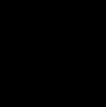
\includegraphics[scale = 0.70]{images/blackbox.png}
            \caption{
        			Black box
        	}
            \label{fig:blackbox}
        \end{figure}

    This is an example of how to cite the figure in the paper. Figure \ref{fig:blackbox} illustrates a sample imported image of a black box. Notice that the \textit{List of Figures} will be generated automatically.


    So far, what do you think? Now, you can start writing your manuscript. I would like you to please read the description in each section to gain an idea of what to write. Please feel free to research online if you need more information.

    \textbf{What is background of the study?}
    The background of the study is a section in a thesis where you provide context and justification for your research. This section typically answers the "why" of your research by explaining the problem or gap in knowledge that your research addresses.

%%%%%%%%%%%%%%%%%%%%%%%%%%%%%%%%%%%%%%%%%%%%%%%%%%%%%%%%%%%%%%%%%%%%%%%
% SECTION 1.2 STATEMENT OF THE PROBLEM
%%%%%%%%%%%%%%%%%%%%%%%%%%%%%%%%%%%%%%%%%%%%%%%%%%%%%%%%%%%%%%%%%%%%%%%
    
\section{Statement of the Problem}
    \label{sec:Statement of the Problem}

    A problem statement is an explanation in research that describes the issue that needs study. What problem is the research attempting to address? It is expected to be brief and concise and should not include the findings of the research or detailed data. It shall define the problem, which can be thought of as a gap in the information base. There may be several solutions to this gap or a need for more information, but that is not the concern of the problem statement. Its purpose is to summarize the current information and where a lack of knowledge may present a problem that must be investigated. The purpose of the problem statement is to identify the issue that is a concern and focus it in a way that allows it to be studied systematically. It defines the problem and demonstrates why further information is needed for a solution to become possible.


%%%%%%%%%%%%%%%%%%%%%%%%%%%%%%%%%%%%%%%%%%%%%%%%%%%%%%%%%%%%%%%%%%%%%%%
% SECTION 1.3 OBJECTIVES OF THE STUDY
%%%%%%%%%%%%%%%%%%%%%%%%%%%%%%%%%%%%%%%%%%%%%%%%%%%%%%%%%%%%%%%%%%%%%%%

\section{Objectives of the Study}
    \label{sec:Objectives of the Study}

    \par The general objective is to . The specific objectives are as follows:
    
    \begin{enumerate}
    	\item To ;
    	\item To ; and
    	\item To .
    \end{enumerate}

%%%%%%%%%%%%%%%%%%%%%%%%%%%%%%%%%%%%%%%%%%%%%%%%%%%%%%%%%%%%%%%%%%%%%%%
% SECTION 1.4 ORIGINALITY OF THE STUDY
%%%%%%%%%%%%%%%%%%%%%%%%%%%%%%%%%%%%%%%%%%%%%%%%%%%%%%%%%%%%%%%%%%%%%%%

\section{Originality of the Study}
\label{sec:Originality of the Study}

    The author should highlight and articulate the unique contributions and novel aspects of the research. This section must differentiate it from the existing literature.


%%%%%%%%%%%%%%%%%%%%%%%%%%%%%%%%%%%%%%%%%%%%%%%%%%%%%%%%%%%%%%%%%%%%%%%
% SECTION 1.5 SCOPES AND LIMITATIONS
%%%%%%%%%%%%%%%%%%%%%%%%%%%%%%%%%%%%%%%%%%%%%%%%%%%%%%%%%%%%%%%%%%%%%%%

\section{Scope and Limitations}
    \label{sec:Scope and Limitations}

    The author needs to outline the boundaries and constraints of the study. This section helps readers understand the extent of the research and the potential limitations that may affect the interpretation of the findings.


%%%%%%%%%%%%%%%%%%%%%%%%%%%%%%%%%%%%%%%%%%%%%%%%%%%%%%%%%%%%%%%%%%%%%%%
% SECTION 1.6 SIGNIFICANCE OF THE STUDY
%%%%%%%%%%%%%%%%%%%%%%%%%%%%%%%%%%%%%%%%%%%%%%%%%%%%%%%%%%%%%%%%%%%%%%%
    
\section{Significance of the Study}
    \label{sec:Significance of the Study}

    For the problem statement being tackled, the results of this study will benefit the following sectors:
    
    \begin{itemize}
        \item\textbf{Benefactor 1}.
         Explain why the study benefits Benefactor 1.
         
    	\item\textbf{Benefactor 2}.
         Explain why the study benefits Benefactor 2.
     
    	\item\textbf{Benefactor 3}.
         Explain why the study benefits Benefactor 3.
    \end{itemize}


%%%%%%%%%%%%%%%%%%%%%%%%%%%%%%%%%%%%%%%%%%%%%%%%%%%%%%%%%%%%%%%%%%%%%%%
% SECTION 1.7 CONCEPTUAL FRAMEWORK
%%%%%%%%%%%%%%%%%%%%%%%%%%%%%%%%%%%%%%%%%%%%%%%%%%%%%%%%%%%%%%%%%%%%%%%

\section{Conceptual Framework}
    \label{sec:Conceptual Framework}
    
    The conceptual framework is a critical research study component that outlines the theoretical foundation and key concepts guiding the investigation. It serves as a roadmap for understanding the relationships between variables and helps researchers formulate hypotheses and design the study. In this section, it is essential to explain the theoretical perspectives, existing models, and relevant literature that inform the study's approach. Additionally, the conceptual framework should elucidate the researcher's assumptions, define key terms, and highlight the conceptual boundaries of the study. By establishing a clear and comprehensive conceptual framework, researchers provide a solid foundation for their work, enabling readers to contextualize the study within the broader academic landscape and grasp the theoretical underpinnings guiding their research endeavors.

    If the study is part of a bigger project, you need to illustrate what portion of the project you are focusing on. You can present the general concept of the project to provide the reader with the big picture. Also, you can present a detailed idea of your study so that it is easy to understand your scope. Please make up your thoughts and divide them by discussing them in different subsections.

    \subsection{Insert Title}
        Lorem Ipsum.
    
    \subsection{Insert Title}
        Lorem Ipsum.


%%%%%%%%%%%%%%%%%%%%%%%%%%%%%%%%%%%%%%%%%%%%%%%%%%%%%%%%%%%%%%%%%%%%%%%
% SECTION 1.8 DEFINITION OF TERMS
%%%%%%%%%%%%%%%%%%%%%%%%%%%%%%%%%%%%%%%%%%%%%%%%%%%%%%%%%%%%%%%%%%%%%%%

\section{Definition of Terms}
    \label{sec:Definition of Terms}

    The following terms are used throughout the study:

    \begin{enumerate}
        \item 
            \textbf{LaTeX} \textemdash is a software system for typesetting documents. It describes the content and layout of the document.
        \item 
            \textbf{Note} \textemdash please arrange your terms alphabetically.
    \end{enumerate}
